\documentclass[11pt]{article}
\usepackage[T1]{fontenc}
\usepackage{lmodern}
\usepackage[expansion=false]{microtype}
\usepackage[margin=1.05in]{geometry}
\usepackage{amsmath,amssymb,amsthm,mathtools}
\usepackage{enumitem,booktabs,array}
\usepackage{needspace}
\usepackage{tikz}
\usetikzlibrary{arrows.meta,positioning}
\PassOptionsToPackage{hyphens}{url}
\usepackage[hidelinks]{hyperref}
\usepackage[nameinlink,capitalize,noabbrev]{cleveref}
\hypersetup{pdftitle={Unitarizability implies amenability for discrete groups},pdfauthor={OpenAI}}
\allowdisplaybreaks[1]
\numberwithin{equation}{section}
\newtheorem{theorem}{Theorem}[section]
\newtheorem{lemma}[theorem]{Lemma}
\newtheorem{proposition}[theorem]{Proposition}
\newtheorem{corollary}[theorem]{Corollary}
\theoremstyle{definition}
\newtheorem{definition}[theorem]{Definition}
\newtheorem{remark}[theorem]{Remark}
\AddToHook{env/theorem/begin}{\crefalias{theorem}{theorem}}
\AddToHook{env/lemma/begin}{\crefalias{theorem}{lemma}}
\AddToHook{env/proposition/begin}{\crefalias{theorem}{proposition}}
\AddToHook{env/corollary/begin}{\crefalias{theorem}{corollary}}
\AddToHook{env/definition/begin}{\crefalias{theorem}{definition}}
\AddToHook{env/remark/begin}{\crefalias{theorem}{remark}}
\newcommand{\C}{\mathbb C}
\newcommand{\R}{\mathbb R}
\newcommand{\Z}{\mathbb Z}
\newcommand{\N}{\mathbb N}
\newcommand{\one}{\mathbf 1}
\newcommand{\HS}{\mathrm{HS}}
\DeclareMathOperator{\Tr}{Tr}
\DeclareMathOperator{\Ad}{Ad}
\DeclareMathOperator{\dist}{dist}
\newcommand{\norm}[1]{\left\lVert#1\right\rVert}
\title{Unitarizability implies amenability for discrete groups}
\author{OpenAI}
\date{September 23, 2026}
\begin{document}
\maketitle
\begin{abstract}
We prove that a discrete group is amenable if and only if every
uniformly bounded representation on a complex Hilbert space is similar
to a unitary representation. This resolves Dixmier's unitarizability
problem affirmatively for discrete groups.
\end{abstract}

\section{Introduction}\label{sec:introduction}

A representation \(\pi:G\to\mathrm{GL}(H)\) of a discrete group on a
complex Hilbert space is \emph{uniformly bounded} if
\[
 |\pi|:=\sup_{g\in G}\norm{\pi(g)}<\infty.
\]
Here \(\mathrm{GL}(H)\) consists of the bounded invertible operators.
The representation is \emph{unitarizable} if some bounded invertible
\(S\) makes every \(S\pi(g)S^{-1}\) unitary. Equivalently, the Hilbert
space admits an equivalent inner product invariant under the
representation. A group is unitarizable when every uniformly bounded
representation on every complex Hilbert space is unitarizable. The
similarity may depend on the representation; its condition number
\(\norm{S}\norm{S^{-1}}\) is not assumed to have a common bound.

A discrete group \(G\) is \emph{amenable} if there is a positive linear
functional \(m:\ell^\infty(G)\to\C\) with \(m(1)=1\) and
\(m(L_gf)=m(f)\), where \((L_gf)(x)=f(g^{-1}x)\).
The one-operator case goes back to Sz.-Nagy: an invertible operator whose
integer powers are uniformly bounded is similar to a unitary operator
\cite[Theorem~I]{SzNagy1947}. His generalized-limit construction of an
invariant inner product preceded the invariant-mean argument of Day and
Dixmier \cite{Day1950,Dixmier1950}. Thus amenability implies
unitarizability. Dixmier explicitly asked whether this property
characterizes groups admitting an invariant mean
\cite[\S5, p.~221]{Dixmier1950}. The question asks whether changing the
Hilbert norm separately for every uniformly bounded representation
already forces the existence of such a mean.

\begin{theorem}\label{thm:main}
A discrete group is amenable if and only if it is unitarizable.
For every discrete nonamenable group \(G\) and every \(\varepsilon>0\),
there are a complex Hilbert space \(\mathcal K\) and a representation
\(\pi:G\to\mathrm{GL}(\mathcal K)\) with \(|\pi|\le1+\varepsilon\)
that is not similar to a unitary representation. If \(G\) is countable,
\(\mathcal K\) may be chosen separable.
\end{theorem}

We work in ZFC. All Hilbert spaces below are complex, and
\(\N=\{1,2,\ldots\}\). The main point is the absence of a similarity for one
representation, without any a priori control on possible similarities.
For an uncountable group the induced witness may be nonseparable, as is
allowed by the definition of unitarizability used here.

\subsection*{Prior work and the remaining obstruction}

Early counterexamples showed that uniform boundedness alone does not
force unitarizability. Ehrenpreis and Mautner constructed examples for
the locally compact group \(\mathrm{SL}_2(\mathbb R)\) \cite{EhrenpreisMautner1955}; explicit
families for free groups include those of Pytlik and Szwarc
\cite{PytlikSzwarc1986}. Nonunitarizability passes from a subgroup to the
ambient group by induction. The free-group examples therefore cover groups
containing nonabelian free subgroups, but leave nonamenable groups
without such subgroups to be understood.

Quantitative unitarizability gives one route to amenability. Pisier
proved that a discrete group \(G\) is amenable exactly when there are
constants \(C\) and \(\alpha<3\), depending only on \(G\), such that
every uniformly bounded representation admits a unitarizer with
condition number at most \(C|\pi|^\alpha\)
\cite[Theorem~0.1]{Pisier1998}. The estimate is uniform over all Hilbert
spaces and representations of the fixed group. Unitarizability itself
implies a polynomial bound of this form for some finite exponent
\cite[Theorem~4.1]{Pisier2004}; the additional content of the amenability
criterion is the threshold \(\alpha<3\).

Random forests gave a route beyond free subgroups. Epstein and Monod
used invariant random forests to relate unitarizability to
\(\ell^2\)-Betti numbers and cost. Their estimates
imply nonunitarizability for residually finite groups with positive
first \(\ell^2\)-Betti number, and for finitely generated residually
finite groups of cost greater than one
\cite[Theorems~1.1--1.3]{EpsteinMonod2009}. Combining their criterion
with group constructions, Osin obtained finitely generated torsion and
torsion-free nonunitarizable groups containing no nonabelian free
subgroup \cite[Theorems~1.2--1.3]{Osin2009}.

A different approach uses measurable actions. Gaboriau and Lyons showed
that a Bernoulli action of a countable nonamenable group contains,
within its orbits, those of an essentially free probability-preserving
action of the free group \(F_2\) \cite[Theorem~1]{GaboriauLyons2009}.
Monod and Ozawa used this to show that, for an
infinite abelian group \(A\), the restricted wreath product
\(A\wr G=(\bigoplus_G A)\rtimes G\) is unitarizable exactly when
\(G\) is amenable \cite[Theorem~1]{MonodOzawa2010}. This places the
obstruction on an extension of \(G\). Alpeev subsequently allowed every
nontrivial countable lamp group \(A\) when \(G\) is countable and
nonamenable, so the conclusion also holds for finite lamps
\cite[Theorem~A]{Alpeev2023}. The distinction remains between a witness
for an extension and one for \(G\) itself.

Approximation properties give a complementary route. Vergara proved
that a discrete unitarizable group satisfying the
\(M_d\)-approximation property for every \(d\ge2\) is amenable.
These conditions hold for countable groups acting properly on
finite-dimensional CAT(0) cube complexes
\cite[Theorems~1.2--1.3]{Vergara2023}. His later extension theorem
preserves \(M_d\)-AP when both a normal subgroup and the quotient
possess it \cite[Theorem~1.3]{Vergara2025}.

Littlewood functions give the analytic formulation closest to the
present proof. Their scalar convolution kernels split into a part with
uniformly absolutely summable rows and a part with uniformly absolutely
summable columns. Epstein and Monod, following Bo\.{z}ejko and Fendler,
use this splitting to obtain bounded commutators and triangular
representations \cite[Propositions~2.3--2.4]{EpsteinMonod2009}.
Gerasimova, Gruber, Monod and Thom relate the corresponding norms to
Cheeger constants and study the resulting restrictions on unitarizable
groups \cite[\S2.B]{GGMT2018}. The passage from bounded non-inner
operator cocycles to nonunitarizable representations is classical
\cite[\S2]{MonodOzawa2010},
\cite[Remark~4 and Proposition~5(ii)]{Pisier2011}.
The present construction retains that mechanism while allowing
finite-dimensional matrix coefficients. Positive rank-one weights
preserve the row and column bounds while increasing the kernel's
Hilbert--Schmidt energy relative to the fibre dimension. This gives a
direct obstruction with no prescribed bound on possible unitarizers.

The passage from countable groups to arbitrary discrete groups uses
standard facts. F\o lner's finite-set criterion implies that every
nonamenable discrete group has a finitely generated nonamenable subgroup
\cite[Main Theorem, p.~245]{Folner1955}.
Induction carries a nonunitarizable representation of that subgroup
to the full group with the same uniform bound
\cite[Proposition~0.5]{Pisier2004}; Pisier's Corollaries~0.10--0.11 also
show that unitarizability of discrete groups is countably determined.

\subsection*{The operator obstruction and the proof}

Let \(U\) be a unitary representation of \(G\) on a Hilbert space
\(\mathcal H\), and write \(\mathcal B(\mathcal H)\) for its bounded
operators. A bounded operator cocycle is a map
\(D:G\to\mathcal B(\mathcal H)\) with
\(\sup_g\norm{D(g)}<\infty\) and
\[
 D(gh)=D(g)+U(g)D(h)U(g)^{-1}.
\]
It is \emph{inner} if one bounded operator \(B\) satisfies
\(D(g)=B-U(g)BU(g)^{-1}\) for all \(g\).
The cocycle gives the uniformly bounded triangular representation
\[
 \pi(g)=\begin{pmatrix}U(g)&D(g)U(g)\\0&U(g)\end{pmatrix}.
\]
A similarity making this representation unitary would produce an
invariant complement to \(\mathcal H\oplus0\). Writing that complement
as the graph of a bounded operator makes \(D\) inner.
Thus it suffices to construct a bounded cocycle with no bounded
implementer.

The criterion in \Cref{sec:obstruction} reduces this task to operators
\(T_j\) on \(\ell^2(G;\C^{k_j})\). Their conjugation differences under
left translation must be bounded uniformly in both \(j\) and \(g\),
while their distance from the operators commuting with left translation
must tend to infinity. A translation-invariant comparison operator
\(A_j\), with blocks \(A_j[x,y]=W_j(x^{-1}y)\), detects that distance:
if the block row at \(e\) of \(T_j\) and the block column at \(e\) of \(A_j-T_j\) have
norm at most \(K\), then
\[
 \dist(T_j,U_j(G)')\ge
 \frac12\left(\frac{\sum_{s\in G}\norm{W_j(s)}_{\HS}^2}{k_j}\right)^{1/2}-K.
\]
Here \(U_j\) is left translation, \(U_j(G)'\) is its commutant, and
\(\norm{W}_{\HS}^2=\operatorname{Tr}(W^*W)\) uses the unnormalized
trace. This estimate compares one finite-dimensional row with one
finite-dimensional column; it imposes no bound on \(\norm{T_j}\).

Nonamenability supplies the operators in two steps. In
\Cref{sec:sparse}, a contracting finite average gives lists
\(s_1,\ldots,s_n\) of group elements, with multiplicity. For \(x\in G\)
and \(1\le i\le n\), the labelled edge \((x,i)\) joins row \(x\) to
column \(xs_i\). These edges can be
assigned to their endpoints so that each endpoint receives at most
\(r\) edges, where \((r/n)\log n\to0\). Compare an assignment with
any left translate. At a row, the edges whose assignment changes lie
in the two sets assigned to that row; at a column, they lie in the
two sets assigned to that column. Thus at most \(2r\) labels change
at either endpoint. In
\Cref{sec:weights}, we choose \(n\) unit vectors in \(\C^k\), with
\(k\) of order \(r\log n\), whose synthesis operators have bounded
norm on every subfamily of at most \(2r\) vectors. This is the
concentration, finite-net and union-bound method familiar from random
matrix estimates; compare \cite[Section~5]{BDDW2008}.
Only its upper norm bound is needed here.

The rank-one projections onto these vectors weight the convolution
edges, and \(T_j\) retains the row-assigned edges. Factoring through
the scalar Hilbert space indexed by the edges
bounds the relevant rows, columns and all conjugation differences.
Keeping the edge labels is essential: distinct products may coincide
in \(G\), yet correspond to distinct coordinates in the factorization.
Positivity ensures that such coincidences do not reduce the kernel
energy, which is at least \(n\). Since \(k/n\to0\), the distance
estimate diverges. Finally, \Cref{sec:conclusion} rescales these operators
and applies the
obstruction to one direct sum of their cocycles, giving any prescribed
uniform bound \(1+\varepsilon\). Induction passes the witness from a
finitely generated nonamenable subgroup to an arbitrary discrete group.
The Day--Dixmier averaging argument completes the equivalence.
\Cref{sec:cstar-consequence} then uses the separate companion similarity
theorem to show that the resulting \(\ell^1(G)\)-representations have no
bounded algebra-homomorphism extension to either group \(C^*\)-algebra.

\section{An invariant-kernel obstruction}
\label{sec:obstruction}

We first prove the criterion announced in the introduction. A large
Hilbert--Schmidt energy will force an operator far from the translation
commutant; a sequence of such operators with uniformly bounded
conjugation differences will then give one bounded non-inner cocycle.
Write $\mathcal B(H)$ for the bounded operators on $H$ and
$\norm{X}_{\HS}^2=\Tr(X^*X)$ for the Hilbert--Schmidt norm of a
finite matrix, with the unnormalized trace $\Tr$.
All operator norms below are ordinary Hilbert-space operator norms.
The finite-dimensional fibres will enter through
Hilbert--Schmidt estimates for one block row and one block column.

For a countable group $G$ and a positive integer $k$, put
\[
  \mathcal H_k=\ell^2(G;\C^k),
  \qquad (U_k(g)\xi)(x)=\xi(g^{-1}x).
\]
For $x\in G$, let $\iota_x:\C^k\to\mathcal H_k$ be the isometric
inclusion into the coordinate indexed by $x$.
For $F\in\mathcal B(\mathcal H_k)$, write
\[
  F[x,y]=\iota_x^*F\iota_y,\qquad
  \operatorname{row}_e(F)=\iota_e^*F,\qquad
  \operatorname{col}_e(F)=F\iota_e.
\]
Thus a block row has codomain $\C^k$ and a block column has domain
$\C^k$. Write $U_k(G)'$ for the bounded operators commuting with
every $U_k(g)$. If $F\in U_k(G)'$, then
$F[x,y]=F[g^{-1}x,g^{-1}y]$, because $U_k(g)\iota_y=\iota_{gy}$.
Taking $g=x$ gives
\[
  F[x,y]=V(x^{-1}y),\qquad V(s)=F[e,s].
\]
This statement concerns the blocks of a bounded operator and requires
no summability assumption on a convolution formula.

\Needspace{18\baselineskip}
\begin{lemma}[Distance from the translation commutant]
\label{lem:kernel-obstruction}
Let $G$ be a countable group, let $k$ be a positive integer, and let
$A,T\in\mathcal B(\mathcal H_k)$ with $A\in U_k(G)'$.
Write
\[
  A[x,y]=W(x^{-1}y),\qquad
  E=\sum_{s\in G}\norm{W(s)}_{\HS}^2.
\]
Suppose that, for some $K\ge0$,
\[
  \norm{\operatorname{row}_e(T)}\le K,
  \qquad
  \norm{\operatorname{col}_e(A-T)}\le K.
\]
Then $E$ is finite and, for every $C\in U_k(G)'$,
\begin{equation}
\label{eq:kernel-energy-obstruction}
  E\le 4k\bigl(K+\norm{T-C}\bigr)^2.
\end{equation}
Consequently,
\begin{equation}
\label{eq:kernel-distance-obstruction}
  \dist\bigl(T,U_k(G)'\bigr)
  \ge \frac12\sqrt{\frac{E}{k}}-K,
\end{equation}
where $\dist(T,U_k(G)')=\inf_{C\in U_k(G)'}\norm{T-C}$.
\end{lemma}

\begin{proof}
Fix $C\in U_k(G)'$, and put
\[
  B=T-C,\qquad h=K+\norm{B},\qquad Q(s)=C[e,s].
\]
The kernel identity above gives $C[x,y]=Q(x^{-1}y)$.
Since $C=T-B$, the operator
\[
  R=\operatorname{row}_e(C):\mathcal H_k\longrightarrow\C^k
\]
has norm at most $h$.
Any bounded operator with codomain $\C^k$ is Hilbert--Schmidt and
has squared Hilbert--Schmidt norm at most $k$ times its squared
operator norm: indeed,
\[
  \norm{R}_{\HS}^2=\Tr(RR^*)\le k\norm{R}^2.
\]
Computing this norm using the coordinate orthonormal basis of
$\mathcal H_k$ therefore gives
\begin{equation}
\label{eq:kernel-row-energy}
  \sum_{s\in G}\norm{Q(s)}_{\HS}^2
  =\norm{R}_{\HS}^2\le kh^2.
\end{equation}

On the other hand, $A-C=(A-T)+B$, so
\[
  L=\operatorname{col}_e(A-C):\C^k\longrightarrow\mathcal H_k
\]
also has norm at most $h$.
Its domain has dimension $k$, whence
\[
  \norm{L}_{\HS}^2=\Tr(L^*L)\le k\norm{L}^2\le kh^2.
\]
The block of this column at row $x$ is
\[
  (A-C)[x,e]=W(x^{-1})-Q(x^{-1}).
\]
Inversion is a bijection of $G$; computing the Hilbert--Schmidt norm
by blocks and reindexing therefore gives
\begin{equation}
\label{eq:kernel-column-energy}
  \sum_{s\in G}\norm{W(s)-Q(s)}_{\HS}^2
  =\norm{L}_{\HS}^2\le kh^2.
\end{equation}
In both computations, the sum of the squared block norms is exactly
the sum of squared matrix coefficients defining the
Hilbert--Schmidt norm.  The group is countable, and all these
summands are nonnegative.

By \Cref{eq:kernel-row-energy,eq:kernel-column-energy}, both $Q$
and $W-Q$ are square summable in the Hilbert--Schmidt norm.
The triangle inequality for these coefficient families gives
\[
  \left(\sum_{s\in G}\norm{W(s)}_{\HS}^2\right)^{1/2}
  \le \sqrt{k}\,h+\sqrt{k}\,h=2\sqrt{k}\,h.
\]
This proves finiteness of $E$ and
\Cref{eq:kernel-energy-obstruction}.
Rearranging that inequality and then taking the infimum over $C$
proves \Cref{eq:kernel-distance-obstruction}.
\end{proof}

The next proposition turns an unbounded sequence of these distances
into one uniformly bounded representation that cannot be
unitarized.  The relation between bounded operator cocycles and
triangular representations is standard; see
\cite[Proposition~2.4]{EpsteinMonod2009},
\cite[Section~2]{MonodOzawa2010}, and
\cite[Remark~4 and Proposition~5(ii)]{Pisier2011}.
We include the argument, in particular the bounded-complement step
and the direct-sum quantifiers.

\begin{proposition}[Direct-sum obstruction]
\label{prop:direct-sum-obstruction}
Let $G$ be a countable group.
For each $j\in\N$, let $k_j$ be a positive integer, put
\[
  \mathcal H_j=\ell^2(G;\C^{k_j}),
  \qquad (U_j(g)\xi)(x)=\xi(g^{-1}x),
\]
and let $A_j,T_j\in\mathcal B(\mathcal H_j)$ with
$A_j\in U_j(G)'$.
Write
\[
  A_j[x,y]=W_j(x^{-1}y),\qquad
  E_j=\sum_{s\in G}\norm{W_j(s)}_{\HS}^2.
\]
Suppose that one constant $K\ge0$ satisfies
\begin{align*}
  \norm{\operatorname{row}_e(T_j)}&\le K, &
  \norm{\operatorname{col}_e(A_j-T_j)}&\le K
  &&(j\in\N),\\
  \norm{T_j-U_j(g)T_jU_j(g)^{-1}}&\le K
  &&&&(j\in\N,\ g\in G).
\end{align*}
Assume also that
\[
  \frac{E_j}{k_j}\longrightarrow\infty.
\]
Then $G$ has a representation on a separable complex Hilbert space
whose operators are bounded and invertible, with
\[
  \sup_{g\in G}\norm{\pi(g)}\le1+K,
\]
and which is not similar to a unitary representation.
No uniform bound on $\norm{T_j}$ or $\norm{A_j}$ is assumed.
\end{proposition}

\begin{proof}
On the Hilbert direct sum
\[
  \mathcal H=\bigoplus_{j\in\N}\mathcal H_j
\]
define
\[
  U(g)=\bigoplus_{j\in\N}U_j(g),\qquad
  D_j(g)=T_j-U_j(g)T_jU_j(g)^{-1},\qquad
  D(g)=\bigoplus_{j\in\N}D_j(g).
\]
The operator $U(g)$ is unitary and $\norm{D(g)}\le K$ by the
hypotheses.  Thus these direct sums are bounded operators on all of
$\mathcal H$.  No bounded operator $\bigoplus_jT_j$ is needed.
Each $\mathcal H_j$ is separable because $G$ is countable and $k_j$
is finite; consequently $\mathcal H$ and $\mathcal H\oplus\mathcal H$
are separable.

Expanding the definition of $D_j$ gives
\[
  D_j(gh)=D_j(g)+U_j(g)D_j(h)U_j(g)^{-1}.
\]
Taking bounded direct sums gives the cocycle identity
\begin{equation}
\label{eq:direct-sum-cocycle}
  D(gh)=D(g)+U(g)D(h)U(g)^{-1}
  \qquad(g,h\in G).
\end{equation}
Define an operator on $\mathcal H\oplus\mathcal H$ by
\begin{equation}
\label{eq:triangular-representation}
  \pi(g)=
  \begin{pmatrix}
    U(g)&D(g)U(g)\\
    0&U(g)
  \end{pmatrix}.
\end{equation}
By \Cref{eq:direct-sum-cocycle}, its upper-right block satisfies
\[
  D(gh)U(gh)
  =D(g)U(g)U(h)+U(g)D(h)U(h).
\]
Multiplication of block matrices now shows
$\pi(g)\pi(h)=\pi(gh)$.
Also $D(e)=0$, so $\pi(e)=\one$.
It follows that each $\pi(g)$ is invertible, with
$\pi(g)^{-1}=\pi(g^{-1})$.
The factorization
\[
  \pi(g)=
  \begin{pmatrix}\one&D(g)\\0&\one\end{pmatrix}
  \begin{pmatrix}U(g)&0\\0&U(g)\end{pmatrix}
\]
has a unitary second factor, whereas the first factor is the
identity plus an operator of norm $\norm{D(g)}$.
Therefore $\norm{\pi(g)}\le1+\norm{D(g)}\le1+K$ for every $g$.

Suppose, for a contradiction, that a bounded invertible operator
$S$ makes $V(g)=S\pi(g)S^{-1}$ unitary for all $g\in G$.
The closed subspace $M=\mathcal H\oplus0$ is invariant under every
$\pi(g)$ and its inverse.  Consequently $SM$ is closed and
invariant under every $V(g)$ and its inverse, so $(SM)^\perp$ is
also invariant.  The subspace
\[
  N=S^{-1}\bigl((SM)^\perp\bigr)
\]
is thus a closed invariant complement of $M$:
$\mathcal H\oplus\mathcal H=M\mathbin{\dotplus}N$.

Let $P_1,P_2:\mathcal H\oplus\mathcal H\to\mathcal H$ be the
coordinate projections.
The restriction $P_2|_N:N\to\mathcal H$ is injective, because
$N\cap M=0$, and surjective, because every $(0,\eta)$ has a
decomposition into an element of $M$ and an element of $N$.
It is a bounded bijection between Banach spaces, hence has bounded
inverse.  Therefore
\[
  B=P_1(P_2|_N)^{-1}\in\mathcal B(\mathcal H),
  \qquad
  N=\{(B\eta,\eta):\eta\in\mathcal H\}.
\]
Applying $\pi(g)$ to this graph and using its invariance gives
\[
  U(g)B\eta+D(g)U(g)\eta=BU(g)\eta
  \qquad(\eta\in\mathcal H).
\]
Since $U(g)$ is invertible, this is equivalent to
\begin{equation}
\label{eq:global-cocycle-implementer}
  D(g)=B-U(g)BU(g)^{-1}.
\end{equation}

Let $I_j:\mathcal H_j\to\mathcal H$ be the canonical isometric
inclusion, and set $B_j=I_j^*BI_j$.
The summand $\mathcal H_j$ reduces every $U(g)$, so
\[
  I_j^*U(g)BU(g)^{-1}I_j
  =U_j(g)B_jU_j(g)^{-1}.
\]
Compressing \Cref{eq:global-cocycle-implementer} therefore yields
\[
  D_j(g)=B_j-U_j(g)B_jU_j(g)^{-1},
  \qquad\norm{B_j}\le\norm{B}.
\]
This compression does not require $B$ to preserve the summands.
Comparison with the definition of $D_j$ shows that
\[
  C_j=T_j-B_j\in U_j(G)'.
\]
Apply \Cref{lem:kernel-obstruction} to $A_j,T_j$ and this choice of
$C_j$.  Its energy estimate gives, for every $j$,
\[
  E_j\le4k_j\bigl(K+\norm{B_j}\bigr)^2
      \le4k_j\bigl(K+\norm{B}\bigr)^2.
\]
This contradicts $E_j/k_j\to\infty$, because $B$ is one bounded
operator.  Hence the representation in
\Cref{eq:triangular-representation} is not similar to a unitary
representation.
\end{proof}

For clarity, each individual $D_j$ in this construction is already
implemented by the bounded operator $T_j$.
The obstruction is to a bounded implementer on the whole direct
sum.  Indeed, \Cref{lem:kernel-obstruction} shows that any operator
$B_j$ satisfying
$D_j(g)=B_j-U_j(g)B_jU_j(g)^{-1}$ for all $g$ must obey
\[
  \norm{B_j}\ge\frac12\sqrt{\frac{E_j}{k_j}}-K.
\]
Thus the proof requires only the existence of a similarity for one
representation in order to obtain a contradiction; it assumes no
uniform bound on similarity operators across different
representations.

\section{Sparse assignments from nonamenability}\label{sec:sparse}

The obstruction requires uniform operator bounds together with increasing
energy per fibre dimension. This section supplies its combinatorial
input: a list of convolution edges that can be assigned to their
endpoints with small loads. The matrix weights in \Cref{sec:weights}
will convert those loads into operator bounds.

Write \((R_tf)(x)=f(xt)\) for right translation on \(\ell^2(G)\).
Thus \(R_sR_t=R_{st}\). We first obtain the finite averaging operator
needed for the construction. This is the elementary averaging-norm
form of the random-walk criterion for nonamenability; compare
\cite{Kesten1959}. We give the implication at the precise strength
used here.

\begin{lemma}\label{lem:contracting-average}
If \(G\) is a nonamenable discrete group, there are a finite set
\(S\subset G\) containing \(e\), with \(d=|S|\ge2\), and a number
\(0<\rho<1\) such that
\[
 \norm{\frac1d\sum_{t\in S}R_t}\le\rho.
\]
\end{lemma}

\begin{proof}
Every such average is a contraction. Suppose all have norm one.
For a unit vector \(f\) and a finite \(S\) of cardinality \(d\),
\[
 \norm{\frac1d\sum_{t\in S}R_tf}_2^2
 =1-\frac1{2d^2}\sum_{t,t'\in S}\norm{R_tf-R_{t'}f}_2^2.
\]
Taking vectors on which the average has norm arbitrarily close to one,
and using \(e\in S\), gives unit vectors arbitrarily close to invariant
under any prescribed finite set of right translations.

For each such vector define the mean
\[
 m_f(b)=\sum_{x\in G}|f(x)|^2b(x^{-1}),\qquad b\in\ell^\infty(G).
\]
Changing variables \(y=xg\) gives
\(m_f(L_gb)=m_{R_{g^{-1}}f}(b)\). The Cauchy--Schwarz inequality yields
\[
 |m_f(L_gb)-m_f(b)|
 \le2\norm{b}_\infty\norm{R_{g^{-1}}f-f}_2.
\]
Direct the finite translation tests and their positive error tolerances
by refinement. A weak-star cluster point of the resulting means exists
by compactness of the dual unit ball. It is positive, normalized, and
left invariant by the displayed estimate. This contradicts
nonamenability. Some average therefore has norm less than one; choose
\(\rho\) between its norm and one. The set has at least two elements,
since the average for \(\{e\}\) is the identity.
\end{proof}

The next argument converts an operator-norm estimate into an assignment
of edges with bounded loads at their endpoints. It is related to the
rectangular kernel estimates for Littlewood functions
\cite[Proposition~2.6]{GGMT2018}; we include the complete assignment
argument and retain all multiplicities. The conversion from endpoint
assignments to row--column bounds also parallels the forest orientation
in \cite[Propositions~2.3--2.4]{EpsteinMonod2009}.

\begin{proposition}\label{prop:sparse-splitting}
Let \(G\) be countable and nonamenable, and fix \(S,d,\rho\) as in
\Cref{lem:contracting-average}. For every \(\ell\ge1\), list the products
of \(\ell\) elements of \(S\), with multiplicity, as
\(s_1,\ldots,s_n\), where \(n=d^\ell\), and put
\(r=\lceil n\rho^\ell\rceil\). There is a function
\(a:G\times\{1,\ldots,n\}\to\{0,1\}\) such that
\begin{equation}\label{eq:sparse-mask}
 \#\{i:a(x,i)=1\}\le r\quad(x\in G),\qquad
 \#\{i:a(ys_i^{-1},i)=0\}\le r\quad(y\in G).
\end{equation}
\end{proposition}

\begin{proof}
The product list satisfies
\[
 \sum_{i=1}^nR_{s_i}=\left(\sum_{t\in S}R_t\right)^\ell,
 \qquad
 \norm{\sum_{i=1}^nR_{s_i}}\le n\rho^\ell.
\]
Consider a bipartite multigraph with row and column vertices in
disjoint copies of \(G\). Its labelled edge \((x,i)\) joins row \(x\)
to column \(xs_i\). For finite row and column sets \(U,V\), pairing
the convolution operator with their indicator functions gives
\begin{equation}\label{eq:edge-count}
 \#\{(x,i):x\in U,\ xs_i\in V\}
 \le n\rho^\ell\sqrt{|U||V|}.
\end{equation}

Give each vertex \(r\) distinct slots. We match every labelled edge to
one slot at one of its two endpoints. For a finite edge set \(F\), let
\(U,V\) be its endpoint sets. Its neighboring slots number
\(r(|U|+|V|)\), whereas \Cref{eq:edge-count} gives
\[
 |F|\le n\rho^\ell\sqrt{|U||V|}
 \le\frac r2(|U|+|V|)\le r(|U|+|V|).
\]
This applies to every finite edge set and hence verifies Hall's
condition for every finite family of edges and all its subfamilies.
For completeness, the finite form of Hall's marriage theorem
\cite{Hall1935} follows here by augmenting paths. Take a matching of maximum
cardinality for a finite family. If an edge-vertex remains unmatched,
follow alternating paths from it. A reachable unmatched slot allows
an augmentation. Otherwise every reachable slot is matched to a
reachable edge-vertex other than the initial one. All neighbors of the
reachable edge-vertices are reachable slots, contradicting Hall's
inequality. Hence every finite family has an injective slot assignment.

Enumerate the countable edge set. The assignments for its finite
initial segments form a tree under restriction, with a node at every
depth and at most \(2r\) extensions of each node. Starting at the root,
choose at each step a child with descendants at arbitrarily large
depths; one exists because there are finitely many children. The
resulting infinite branch supplies a simultaneous assignment. Set \(a(x,i)=1\) when the edge is assigned to
its row and zero when it is assigned to its column. No vertex receives
more than \(r\) edges, proving \Cref{eq:sparse-mask}. Parallel edges
remain distinct throughout the matching, and the two endpoints remain
distinct vertices even if \(s_i=e\).
\end{proof}

\section{Finite-dimensional weights and sparse block operators}
\label{sec:weights}

The sparse assignment from \Cref{sec:sparse} will now produce the three
bounds required by \Cref{prop:direct-sum-obstruction}: a bound on each
block row of \(T\), each block column of \(A-T\), and every conjugation
difference \(T-U(g)TU(g)^{-1}\). All three bounds will be independent
of the number of labels. To make the energy grow faster than the fibre
dimension, we use rank-one projections onto many unit vectors in a
smaller space.

We first construct vectors whose synthesis operators are bounded on
every small subfamily. The proof uses the standard concentration,
finite-net and union-bound method for random matrices; compare
\cite[Section~5]{BDDW2008}. Here only an upper bound is needed, and the
argument below supplies its constants directly.

\begin{lemma}[An upper bound for all small subfamilies]
\label{lem:frames}
Let $n\ge 2$ and $r\ge 1$ be integers, and put
\begin{equation}
\label{eq:frame-parameters}
 p=\min(2r,n),\qquad
 k=\left\lceil 2r\log(2n)\right\rceil,
 \qquad b_0=10,
\end{equation}
where $\log$ denotes the natural logarithm.  There are unit vectors
$v_1,\ldots,v_n\in\C^k$ such that, for every
$J\subseteq\{1,\ldots,n\}$ with $|J|\le p$, the operator
\[
 V_J\colon\ell^2(J)\longrightarrow\C^k,
 \qquad V_J z=\sum_{i\in J}z_i v_i,
\]
satisfies $\norm{V_J}\le b_0$.
\end{lemma}

\begin{proof}
Choose independent random variables $\varepsilon_{a,i}$, for
$1\le a\le k$ and $1\le i\le n$, each taking the values $1$ and $-1$
with probability $1/2$, and set
\[
 (v_i)_a=k^{-1/2}\varepsilon_{a,i}.
\]
Every $v_i$ has norm exactly one.  Fix a set
$J=\{i_1<\cdots<i_p\}$ of cardinality $p$, and fix real unit vectors
$w\in\mathbb R^k$ and $z\in\mathbb R^p$.  The random variable
\[
 X=w^{\mathsf T}V_Jz
   =\frac1{\sqrt{k}}
     \sum_{a=1}^k\sum_{j=1}^p w_a z_j\varepsilon_{a,i_j}
\]
is a sum of independent signs with deterministic coefficients whose
squares sum to
\[
 \frac1k\sum_{a=1}^k\sum_{j=1}^p w_a^2z_j^2=\frac1k.
\]
The inequality $\cosh t\le\exp(t^2/2)$ consequently gives, for every
$t\in\mathbb R$,
\[
 \mathbb E\exp(tX)
 =\prod_{a,j}\cosh\!\left(\frac{t w_a z_j}{\sqrt{k}}\right)
 \le\exp\!\left(\frac{t^2}{2k}\right).
\]
For $u>0$, applying Markov's inequality to $\exp(tX)$ and choosing
$t=ku$ yields $\Pr(X>u)\le\exp(-ku^2/2)$.  The same argument for
$-X$ therefore proves
\begin{equation}
\label{eq:sign-tail}
 \Pr(|X|>u)\le 2\exp(-ku^2/2).
\end{equation}
In particular, the probability that $|X|>5$ is at most
$2\exp(-25k/2)$.

For each positive integer $m$, the real Euclidean unit sphere has a
$1/4$-net with at most $9^m$ points.  Indeed, take a maximal
$1/4$-separated set on that sphere.  The open balls of radius $1/8$
about its points are pairwise disjoint and lie in the ball of radius
$9/8$ about the origin.  Comparing their $m$-dimensional volumes bounds
the number of points by $9^m$.  Maximality makes the set a $1/4$-net.

Fix such nets $\mathcal N_k\subset\mathbb R^k$ and
$\mathcal N_p\subset\mathbb R^p$.  For any real $k\times p$ matrix
$M$, let $L$ be its operator norm on real Euclidean spaces.  If
$|w_0^{\mathsf T}Mz_0|\le5$ for all
$(w_0,z_0)\in\mathcal N_k\times\mathcal N_p$, then, for arbitrary
real unit vectors $w,z$, choose net points satisfying
$\norm{w-w_0}\le1/4$ and $\norm{z-z_0}\le1/4$.  We obtain
\[
 \left|w^{\mathsf T}Mz-w_0^{\mathsf T}Mz_0\right|
 \le \norm{w-w_0}L\norm{z}
       +\norm{w_0}L\norm{z-z_0}
 \le\frac L2.
\]
Taking the supremum over $w,z$ gives $L\le5+L/2$, hence $L\le10$.

There are at most $n^p$ sets $J$ of size $p$.  By
\Cref{eq:sign-tail} and the union bound, the probability that one of
the corresponding net inequalities fails is at most
\begin{equation}
\label{eq:frame-failure-probability}
 2n^p9^{k+p}\exp(-25k/2).
\end{equation}
The parameters satisfy
\[
 k\ge2r\log(2n)\ge p,
 \qquad k\ge p\log n.
\]
Here $\log(2n)\ge\log4>1$ and $p\le2r$.  Thus the logarithm of
the bound in \Cref{eq:frame-failure-probability} is at most
\[
 \log2+k+2k\log9-\frac{25k}{2}
 =\log2-\left(\frac{25}{2}-1-2\log9\right)k<0.
\]
For example, the coefficient in parentheses exceeds $7$, whereas
$k\ge1$ and $\log2<1$.  The bound in
\Cref{eq:frame-failure-probability} is therefore strictly less than
one.  There is a realization for which every size-$p$ synthesis
matrix has real operator norm at most $10$.

For a real matrix $M$ with real operator norm $L$, and real vectors
$u,v$, one has
\[
 \norm{M(u+iv)}^2=\norm{Mu}^2+\norm{Mv}^2
 \le L^2\bigl(\norm{u}^2+\norm{v}^2\bigr).
\]
Since real vectors are also complex vectors, this proves equality of
the real and complex operator norms.  The realization just obtained
therefore has the claimed complex operator norm bounds.  Finally,
every set with fewer than $p$ indices is contained in one with $p$
indices, and its synthesis operator is the restriction to a coordinate
subspace of that larger synthesis operator.  This proves the assertion
for all $|J|\le p$.
\end{proof}

The vectors just constructed control each small set of incident labels.
We next transfer that finite-dimensional estimate to an operator on the
group. The intermediate space keeps one scalar coordinate for each
labelled edge, even when several labels describe the same group element.

\subsection{A factorization through the indexed edges}

Let $G$ be a countable group, let $s_1,\ldots,s_n\in G$ be a finite
list, and allow the same group element to occur at several distinct
indices.  Let $v_1,\ldots,v_n\in\C^k$ be unit vectors and put
\[
 P_i=v_i v_i^*,\qquad
 \mathcal H=\ell^2(G;\C^k).
\]
Thus $P_i$ is a rank-one orthogonal projection and
$\norm{P_i}=1$.  For a function
$c\colon G\times\{1,\ldots,n\}\to\C$ with $|c(x,i)|\le1$, define
\begin{equation}
\label{eq:masked-operator}
 (T_c\xi)(x)=\sum_{i=1}^n c(x,i)P_i\xi(xs_i),
 \qquad \xi\in\mathcal H.
\end{equation}
For each fixed $i$, the corresponding summand is the composition of
the unitary right shift $\xi(x)\mapsto\xi(xs_i)$, the pointwise
application of $P_i$, and multiplication by the scalar function
$c(\cdot,i)$.  Its norm is at most one.  In particular,
\Cref{eq:masked-operator} defines a bounded operator and
$\norm{T_c}\le n$, without any sparsity assumption.  The next lemma
gives a bound independent of $n$ under two sparsity assumptions.

\begin{lemma}[The masked operator estimate]
\label{lem:masked}
In the preceding setting, let $1\le p\le n$ and $b_0>0$.  Suppose
that
\[
 \norm{V_J}\le b_0
 \quad\text{for every }J\subseteq\{1,\ldots,n\}
 \text{ with }|J|\le p,
\]
where $V_J$ is the synthesis operator with columns $v_i$, $i\in J$.
For a mask $c$ as in \Cref{eq:masked-operator}, define
\[
 \mathcal R_x=\{i:c(x,i)\ne0\},\qquad
 \mathcal C_y=\{i:c(ys_i^{-1},i)\ne0\}.
\]
If $|\mathcal R_x|\le p$ for every $x\in G$ and $|\mathcal C_y|\le p$ for every
$y\in G$, then
\[
 \norm{T_c}\le b_0^2.
\]
\end{lemma}

\begin{proof}
Keep the index $i$ as part of each edge and set
\[
 E_c=\{(x,i):c(x,i)\ne0\},
 \qquad \mathcal E_c=\ell^2(E_c).
\]
Define the analysis operator $F\colon\mathcal H\to\mathcal E_c$,
the diagonal multiplication operator
$M_c\colon\mathcal E_c\to\mathcal E_c$, and the synthesis operator
$S\colon\mathcal E_c\to\mathcal H$ by
\begin{align*}
 (F\xi)(x,i)&=v_i^*\xi(xs_i),\\
 (M_c\alpha)(x,i)&=c(x,i)\alpha(x,i),\\
 (S\alpha)(x)&=\sum_{i\in \mathcal R_x}v_i\alpha(x,i).
\end{align*}
Figure~\ref{fig:edge-factorization} illustrates the role of the edge
coordinates. The following estimates both justify these operators on the
stated Hilbert spaces and bound their norms.
\begin{figure}[tb]
\centering
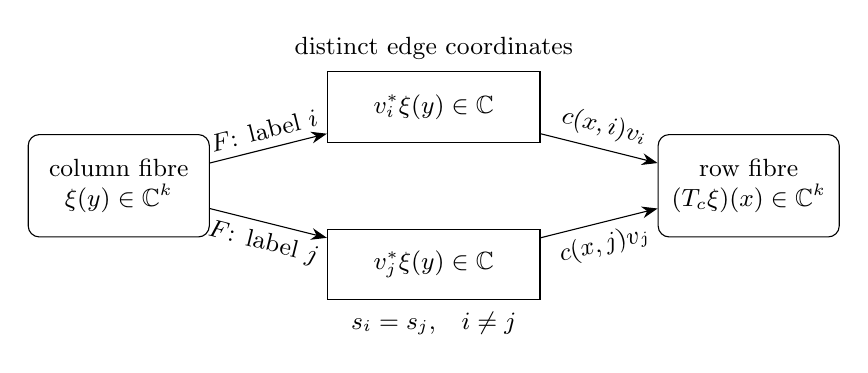
\begin{tikzpicture}[
  >={Stealth[length=2mm]},
  fibre/.style={draw,rounded corners,minimum width=23mm,minimum height=13mm,align=center},
  edgecoord/.style={draw,minimum width=27mm,minimum height=9mm,align=center},
  every node/.style={font=\small}]
\node[fibre] (column) at (0,0) {column fibre\\$\xi(y)\in\C^k$};
\node[edgecoord] (ei) at (4,1) {$v_i^*\xi(y)\in\C$};
\node[edgecoord] (ej) at (4,-1) {$v_j^*\xi(y)\in\C$};
\node[fibre] (row) at (8,0) {row fibre\\$(T_c\xi)(x)\in\C^k$};
\draw[->] (column) -- node[above,sloped] {$F$: label $i$} (ei);
\draw[->] (column) -- node[below,sloped] {$F$: label $j$} (ej);
\draw[->] (ei) -- node[above,sloped] {$c(x,i)v_i$} (row);
\draw[->] (ej) -- node[below,sloped] {$c(x,j)v_j$} (row);
\node at (4,1.75) {distinct edge coordinates};
\node at (4,-1.75) {$s_i=s_j$,\quad $i\ne j$};
\end{tikzpicture}

\caption{Two different labels with \(s_i=s_j\) give parallel edges from
row \(x\) to column \(y=xs_i=xs_j\). The operator acts from the column
fibre toward the row fibre. Analysis produces separate scalar
coordinates \((x,i)\) and \((x,j)\); multiplication by the mask and
synthesis then add their contributions in the row fibre. The picture
shows only these two coordinates of the factorization \(T_c=SM_cF\).}
\label{fig:edge-factorization}
\end{figure}  For $S$, the row assumption gives
\[
 \norm{S\alpha}^2
 =\sum_x\norm{V_{\mathcal R_x}(\alpha(x,i))_{i\in \mathcal R_x}}^2
 \le b_0^2\sum_x\sum_{i\in \mathcal R_x}|\alpha(x,i)|^2
 =b_0^2\norm{\alpha}^2.
\]
For $F$, regroup the nonnegative summands by the column $y=xs_i$.
For fixed $y$ and fixed label $i$, there is exactly one possible
source, namely $x=ys_i^{-1}$.  The edges arriving at $y$ are
therefore indexed by the set $\mathcal C_y$, with no repeated index, and
\begin{align*}
 \norm{F\xi}^2
 &=\sum_y\sum_{i\in \mathcal C_y}|v_i^*\xi(y)|^2\\
 &=\sum_y\norm{V_{\mathcal C_y}^*\xi(y)}^2
 \le b_0^2\sum_y\norm{\xi(y)}^2
 =b_0^2\norm{\xi}^2.
\end{align*}
Empty index sets contribute zero in both calculations.  These
estimates give $\norm{S}\le b_0$ and $\norm{F}\le b_0$, and
$|c(x,i)|\le1$ gives $\norm{M_c}\le1$.  Substitution into the
definitions yields the exact factorization
\[
 T_c=S M_c F.
\]
Consequently $\norm{T_c}\le b_0^2$.

The uniqueness of $x=ys_i^{-1}$ uses a fixed label $i$, not the
distinctness of the elements in the list $s_1,\ldots,s_n$.
In particular, if $s_i=s_j$ for $i\ne j$, the two indexed edges remain
distinct coordinates of $\mathcal E_c$.  Their contributions to a
common operator block are summed by the same factorization.  No
distinctness assumption on the products is needed.
\end{proof}

\subsection{Consequences of an assignment to endpoints}

We now apply the factorization three times to obtain the hypotheses of
\Cref{prop:direct-sum-obstruction}. An endpoint assignment is sparse
only for the ones at rows and the zeros at columns. Restricting to a
single row or column, and then subtracting a translated assignment,
will give masks that are sparse on both sides.

Fix integers $n\ge2$ and $r\ge1$, and choose $k,p,b_0$ and
$v_1,\ldots,v_n$ as in \Cref{lem:frames}.  Keep the preceding
notation $G,s_i,P_i,\mathcal H,T_c$.  Suppose a function
$a\colon G\times\{1,\ldots,n\}\to\{0,1\}$ satisfies
\begin{equation}
\label{eq:weights-orientation-bounds}
 \sum_{i=1}^n a(x,i)\le r\quad(x\in G),
 \qquad
 \sum_{i=1}^n\bigl(1-a(ys_i^{-1},i)\bigr)\le r\quad(y\in G).
\end{equation}
Thus the ones are sparse at rows and the zeros are sparse at columns,
with both counts taken over indexed edges.  Set
\begin{equation}
\label{eq:weights-A-T-U}
 A=T_{\one},\qquad T=T_a,\qquad
 (U(g)\xi)(x)=\xi(g^{-1}x)\quad(g,x\in G),
\end{equation}
where $\one(x,i)=1$.  Both $A$ and $T$ are bounded operators, each
with norm at most $n$. For $y\in G$, let
$\iota_y:\C^k\to\mathcal H$ be the coordinate inclusion, and write
$q_y=\iota_y^*$ for coordinate evaluation.

\begin{corollary}[Individual block rows and columns]
\label{cor:block-rows-columns}
Under \Cref{eq:weights-orientation-bounds}, one has
\[
 \norm{q_xT}\le b_0^2\quad(x\in G),
 \qquad
 \norm{(A-T)\iota_y}\le b_0^2\quad(y\in G).
\]
\end{corollary}

\begin{proof}
Write $\one_E$ for the indicator of a condition $E$.
For fixed $x_0,y_0\in G$, define the masks
\[
 c_{\mathrm r}(x,i)=\one_{\{x=x_0\}}a(x,i),\qquad
 c_{\mathrm c}(x,i)=\one_{\{xs_i=y_0\}}(1-a(x,i)).
\]
The first inequality in \Cref{eq:weights-orientation-bounds} gives
at most $r$ active edges in total for $c_{\mathrm r}$; the second
gives the same bound for $c_{\mathrm c}$.
Thus every row and every column of either mask has at most
$\min(r,n)\le p$ active indices, and \Cref{lem:masked} bounds both
associated operator norms by $b_0^2$. Their operators are
\[
 T_{c_{\mathrm r}}=\iota_{x_0}q_{x_0}T,\qquad
 T_{c_{\mathrm c}}=(A-T)\iota_{y_0}q_{y_0}.
\]
The first norm equals $\norm{q_{x_0}T}$ because $\iota_{x_0}$ is
isometric. The second equals $\norm{(A-T)\iota_{y_0}}$ because
$\norm{q_{y_0}}=1$ and $q_{y_0}\iota_{y_0}=I_{\C^k}$.
These are the asserted bounds.
\end{proof}

\begin{proposition}[Uniformly bounded conjugation differences]
\label{prop:uniform-differences}
Under \Cref{eq:weights-orientation-bounds}, the maps $U(g)$ in
\Cref{eq:weights-A-T-U} form a unitary representation of $G$,
and $A$ commutes with every $U(g)$.  Define
\[
 D(g)=T-U(g)TU(g)^{-1}\quad(g\in G).
\]
Then
\begin{equation}
\label{eq:uniform-difference-bound}
 \sup_{g\in G}\norm{D(g)}\le b_0^2=100.
\end{equation}
Moreover, $D(e)=0$ and
\begin{equation}
\label{eq:weights-cocycle}
 D(gh)=D(g)+U(g)D(h)U(g)^{-1}\quad(g,h\in G).
\end{equation}
\end{proposition}

\begin{proof}
Left multiplication by a group element is a bijection of $G$, so
each $U(g)$ is unitary with inverse $U(g^{-1})$, and direct
substitution gives $U(g)U(h)=U(gh)$.
Left and right translations
commute and $U(g)$ acts trivially on the fibre $\C^k$; alternatively,
direct substitution in \Cref{eq:masked-operator} with $c=\one$
gives $U(g)A=AU(g)$.

For a general mask $a$, direct calculation gives
\[
 (U(g)TU(g)^{-1}\xi)(x)
 =\sum_{i=1}^n a(g^{-1}x,i)P_i\xi(xs_i).
\]
Thus $D(g)=T_{c_g}$ for the mask
\[
 c_g(x,i)=a(x,i)-a(g^{-1}x,i)\in\{-1,0,1\}.
\]
At any row $x$, the active indices are contained in
\[
 \{i:a(x,i)=1\}\ \cup\ \{i:a(g^{-1}x,i)=1\}.
\]
Each set in this union has at most $r$ elements by
\Cref{eq:weights-orientation-bounds}.  Hence there are at most
$\min(2r,n)=p$ active indices at that row.

For the column estimate, write
\[
 Z_y=\{i:a(ys_i^{-1},i)=0\}\quad(y\in G).
\]
The second inequality in \Cref{eq:weights-orientation-bounds}
gives $|Z_y|\le r$.  The active indices of $c_g$ at a column $y$
are precisely those for which
\[
 a(ys_i^{-1},i)\ne a(g^{-1}ys_i^{-1},i).
\]
Since $a$ takes only the values zero and one, this set is
$Z_y\mathbin\triangle Z_{g^{-1}y}$, the symmetric difference of
the two zero sets.  It has at most $2r$ elements, and at most $n$,
so its cardinality is at most $p$.  As in \Cref{lem:masked},
fixed $y$ and fixed label $i$ specify the unique source
$ys_i^{-1}$.  These counts therefore concern exactly the indexed
edges of the mask, including when products coincide.

Both hypotheses of \Cref{lem:masked} now hold for $c_g$, and
$|c_g(x,i)|\le1$.  That lemma yields
$\norm{D(g)}\le b_0^2$ for every $g$, proving
\Cref{eq:uniform-difference-bound}.

Finally, $D(e)=T-T=0$. The cocycle identity in
\Cref{eq:weights-cocycle} follows from the calculation in the proof
of \Cref{prop:direct-sum-obstruction}.
\end{proof}

\section{Proof of the main theorem}\label{sec:conclusion}

We first combine the three uniform bounds with the kernel energy estimate
for countable groups. We then pass through a finitely generated subgroup
to arbitrary discrete groups and include the classical averaging argument
for the reverse direction.

\begin{proof}[The countable nonamenable case]
Fix a countable discrete nonamenable group \(G\), and choose
\(S,d,\rho\) from \Cref{lem:contracting-average}.
For each \(\ell\ge1\), take the product list and assignment of
\Cref{prop:sparse-splitting}, with
\[
 n_\ell=d^\ell,\qquad
 r_\ell=\lceil n_\ell\rho^\ell\rceil,\qquad
 k_\ell=\lceil2r_\ell\log(2n_\ell)\rceil.
\]
In particular,
\begin{equation}\label{eq:dimension-ratio}
 \frac{k_\ell}{n_\ell}
 \le2\left(\rho^\ell+\frac1{n_\ell}\right)\log(2n_\ell)
       +\frac1{n_\ell}\longrightarrow0.
\end{equation}
Choose the vectors from \Cref{lem:frames} and let
\(P_i=v_iv_i^*\) at this stage. Use them to form the operators
\(A_\ell,T_\ell,U_\ell\) of \Cref{sec:weights} on
\(\mathcal H_\ell=\ell^2(G;\C^{k_\ell})\).
The row and column bounds of \Cref{cor:block-rows-columns} and the
commutator bound of \Cref{prop:uniform-differences} have the common
constant \(K=b_0^2=100\).

The invariant kernel of \(A_\ell\) is
\[
 W_\ell(s)=\sum_{i:s_i=s}P_i.
\]
It is finitely supported. Positivity of the weights gives
\begin{equation}\label{eq:kernel-energy}
 \sum_{s\in G}\norm{W_\ell(s)}_{\HS}^2
 =\sum_{i,j:s_i=s_j}\Tr(P_iP_j)
 =\sum_{i,j:s_i=s_j}|v_i^*v_j|^2
 \ge n_\ell.
\end{equation}
The diagonal terms equal one, and every other term is nonnegative;
thus collisions among group products only increase this lower bound.
By \Cref{eq:dimension-ratio}, the kernel energy divided by
\(k_\ell\) tends to infinity.

Fix \(\varepsilon>0\) and put \(t=\varepsilon/100\). Apply
\Cref{prop:direct-sum-obstruction} to the rescaled operators
\(tA_\ell,tT_\ell\). Their three uniform bounds have the common
constant \(tK=\varepsilon\). Their invariant kernels are
\(tW_\ell\), so their energies divided by \(k_\ell\) still tend to
infinity: they are \(t^2\) times the ratios just established.
The proposition therefore gives a representation on
\[
 \mathcal K=
 \left(\bigoplus_{\ell\ge1}\mathcal H_\ell\right)
 \oplus\left(\bigoplus_{\ell\ge1}\mathcal H_\ell\right)
\]
with uniform bound at most \(1+\varepsilon\) that is not similar to a
unitary representation. This Hilbert space is separable because \(G\)
is countable and each \(k_\ell\) is finite. This proves the nonamenable
direction and the quantitative assertion for countable groups.
\end{proof}

We next recall the induction argument for subgroup permanence of
unitarizability \cite[Proposition~0.5]{Pisier2004}, keeping track of its
norm and of the invariant inner product on the subgroup representation.

\begin{lemma}[Induction from a subgroup]\label{lem:subgroup-induction}
Let \(H\) be a subgroup of a discrete group \(G\), and let
\(\sigma:H\to\mathrm{GL}(\mathcal K)\) be a uniformly bounded
representation on a complex Hilbert space. There is a uniformly bounded
representation \(\Pi:G\to\mathrm{GL}(\mathcal L)\) on
\(\mathcal L=\ell^2(G/H;\mathcal K)\) such that
\[
 |\Pi|=|\sigma|.
\]
If \(\Pi\) is unitarizable, then \(\sigma\) is unitarizable.
\end{lemma}

\begin{proof}
Write \(X=G/H\) for the left cosets, and choose representatives
\(s:X\to G\) with \(s(H)=e\). For \(g\in G\) and \(x\in X\), put
\[
 c(g,x)=s(gx)^{-1}g s(x)\in H.
\]
The membership follows because \(s(gx)H=gs(x)H\). Direct multiplication
gives
\[
 c(gh,x)=c(g,hx)c(h,x)\qquad(g,h\in G,\ x\in X).
\]
On the dense subspace of finitely supported families in the Hilbert
direct sum \(\mathcal L=\bigoplus_{x\in X}\mathcal K\), define
\[
 (\Pi(g)\xi)_{gx}=\sigma(c(g,x))\xi_x\qquad(x\in X).
\]
If \(M=|\sigma|\), then reindexing by the permutation \(x\mapsto gx\)
gives
\[
 \norm{\Pi(g)\xi}^2
 =\sum_{x\in X}\norm{\sigma(c(g,x))\xi_x}^2
 \le M^2\sum_{x\in X}\norm{\xi_x}^2.
\]
Thus \(\Pi(g)\) extends to a bounded operator of norm at most \(M\) on
the whole direct sum, without a countability assumption on \(X\).
The cocycle identity gives \(\Pi(g)\Pi(h)=\Pi(gh)\) first on finitely
supported families and hence everywhere. Also \(\Pi(e)=I\), so
\(\Pi(g)^{-1}=\Pi(g^{-1})\). This proves \(|\Pi|\le M\).

Let \(j:\mathcal K\to\mathcal L\) be the isometric inclusion at the
identity coset \(H\). For \(h\in H\), one has \(hH=H\) and
\(c(h,H)=h\), whence
\[
 \Pi(h)j=j\sigma(h).
\]
In particular, \(\norm{\Pi(h)}\ge\norm{\sigma(h)}\) for every
\(h\in H\). Taking suprema gives the reverse inequality
\(|\Pi|\ge|\sigma|\), proving equality of the uniform bounds.

Suppose now that \([\cdot,\cdot]\) is an invariant equivalent inner
product for \(\Pi\). Let \(Q\) be the bounded positive invertible operator
representing this form. It satisfies
\[
 aI\le Q\le bI,\qquad \Pi(g)^*Q\Pi(g)=Q\quad(g\in G)
\]
for some \(0<a\le b<\infty\). The compression \(Q_H=j^*Qj\) satisfies
\[
 aI\le Q_H\le bI,\qquad
 \sigma(h)^*Q_H\sigma(h)
 =j^*\Pi(h)^*Q\Pi(h)j=Q_H\quad(h\in H).
\]
Consequently \([v,w]_H=[jv,jw]\) is an equivalent
\(\sigma(H)\)-invariant inner product on \(\mathcal K\). The compression
does not require \(Q\) to preserve the identity-coset summand. Hence
\(\sigma\) is unitarizable.
\end{proof}

\begin{proof}[Arbitrary discrete nonamenable groups]
Let \(G\) be a discrete nonamenable group and fix \(\varepsilon>0\).
The F\o lner criterion for an arbitrary discrete group says that
amenability is equivalent to the following condition: for every finite
\(S\subseteq G\) and every \(\delta>0\), there is a finite nonempty
\(F\subseteq G\) such that
\begin{equation}\label{eq:folner-finite-test}
 |sF\mathbin\triangle F|<\delta|F|\qquad(s\in S).
\end{equation}
This is the symmetric-difference form of F\o lner's Main Theorem
\cite[p.~245]{Folner1955}: inversion exchanges right and left
translations, and \(|sF\mathbin\triangle F|=2(|F|-|sF\cap F|)\).
No F\o lner sequence is required.

Since \(G\) is nonamenable, some finite \(S\) and positive \(\delta\)
fail this condition. The subgroup \(H=\langle S\rangle\) is finitely
generated and therefore countable. It is nonamenable: otherwise the
criterion applied inside \(H\) would give a finite nonempty
\(F\subseteq H\) satisfying \Cref{eq:folner-finite-test}, and the same
inequalities would hold in \(G\), a contradiction.

The countable case proved above gives a nonunitarizable
representation \(\sigma\) of \(H\) on a separable Hilbert space with
\(|\sigma|\le1+\varepsilon\). By Lemma~\ref{lem:subgroup-induction}, its
induced representation \(\Pi\) of \(G\) has
\(|\Pi|=|\sigma|\le1+\varepsilon\) and is nonunitarizable. This proves
the nonamenable direction for every discrete group.
\end{proof}

\begin{proof}[The amenable direction]
Let \(G\) be amenable and let \(\pi:G\to\mathrm{GL}(H)\) be uniformly
bounded, with \(M=|\pi|\). The Day--Dixmier argument
\cite{Day1950,Dixmier1950} works on an arbitrary complex Hilbert space.
If \(m\) is a left invariant mean, then
\(m_{\mathrm r}(f)=m(x\mapsto f(x^{-1}))\) is a right invariant mean.
Define a sesquilinear form by
\[
 [\xi,\eta]=m_{\mathrm r}\bigl(g\mapsto
                 \langle\pi(g)\xi,\pi(g)\eta\rangle\bigr).
\]
Since both \(\norm{\pi(g)}\) and \(\norm{\pi(g)^{-1}}\) are at most
\(M\), positivity of the mean gives
\[
 M^{-2}\norm{\xi}^2\le[\xi,\xi]\le M^2\norm{\xi}^2.
\]
Thus this is an equivalent Hilbert inner product. Right invariance
gives \([\pi(h)\xi,\pi(h)\eta]=[\xi,\eta]\) for every \(h\in G\).
Representing the form by a bounded positive invertible operator \(Q\),
we have \(\pi(h)^*Q\pi(h)=Q\). Hence \(S=Q^{1/2}\) is bounded and
invertible, and \(S\pi(h)S^{-1}\) is unitary for all \(h\). This proves
unitarizability and completes the equivalence.
\end{proof}

For uncountable nonamenable \(G\), the finitely generated subgroup \(H\) above has
uncountable index, and the induced witness is nonseparable. The conclusion
therefore uses the usual definition quantifying over all Hilbert spaces.
The argument concerns discrete groups and does not extend the theorem to
nondiscrete locally compact groups, where representations are normally
required to be strongly continuous.

\section{A consequence for group \texorpdfstring{$C^*$}{C*}-algebras}
\label{sec:cstar-consequence}

The following consequence uses the companion similarity theorem in
addition to \Cref{thm:main}.

Let \(G\) be any discrete group and let
\(\pi:G\to\mathrm{GL}(H)\) be a uniformly bounded nonunitarizable
representation on a complex Hilbert space. The operator-norm convergent sum
\[
 T_\pi(f)=\sum_{g\in G}f(g)\pi(g),\qquad f\in\ell^1(G),
\]
defines a bounded complex-linear unital homomorphism for convolution, with
\(\norm{T_\pi(f)}\le|\pi|\norm{f}_1\); absolute summability justifies
multiplication of the sums. Nevertheless, its restriction to \(\C[G]\)
has no bounded complex-linear unital algebra-homomorphism extension to
either the full group algebra \(C^*(G)\) or the reduced group algebra
\(C_r^*(G)\). Indeed, a full extension \(\Phi\) would be similar to a
\(*\)-homomorphism by the companion similarity theorem
\cite[Theorem~1.1]{OpenAIKadison2026}: some bounded invertible \(S\)
would make \(S\Phi(\cdot)S^{-1}\) a unital \(*\)-homomorphism.
For each canonical group unitary \(u_g\), one has \(\Phi(u_g)=\pi(g)\),
so every \(S\pi(g)S^{-1}\) would be unitary, a contradiction.
A reduced extension would compose with the canonical unital
\(*\)-quotient \(C^*(G)\to C_r^*(G)\) to give a full extension.
Thus the automatic \(\ell^1\)-norm bound does not imply
\(C^*\)-norm continuity. Applying this observation to the witnesses in
\Cref{thm:main} gives such a failure for every nonamenable discrete
group, even with uniform representation bounds arbitrarily close to one.


\begingroup
\raggedright
\let\standardbibliography\thebibliography
\renewcommand{\thebibliography}[1]{%
  \standardbibliography{#1}\setlength{\itemsep}{3pt}}
\bibliographystyle{plain}
\bibliography{references}
\endgroup
\end{document}
